\documentclass{article}

\usepackage[english]{babel}
\usepackage[a4paper, top=2cm, bottom=2cm, left=3cm, right=3cm, marginparwidth=1.75cm]{geometry}
\usepackage{graphicx}
\usepackage{subfigure}

\title{Ribosomes}
\author{Anamaria Hodivoianu, Class 332}

\begin{document}
\maketitle

\section{Definition}
Ribosomes are "machines" responsible for synthesizing proteins. They exist in both prokaryotic and eukaryotic cells, with some differences between the two types. Ribosomes have two subunits, a large and a small one, each with its own role, that become joined during the protein synthesis process. Ribosomes are made up of ribosomal RNA (rRNA) and proteins.

\begin{figure}
    \centering
    \subfigure{
        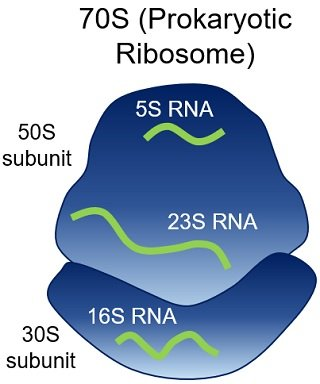
\includegraphics[width=0.2\textwidth]{70-S-ribosome.jpg}
    }
    \hspace{0.05\textwidth}
    \subfigure{
        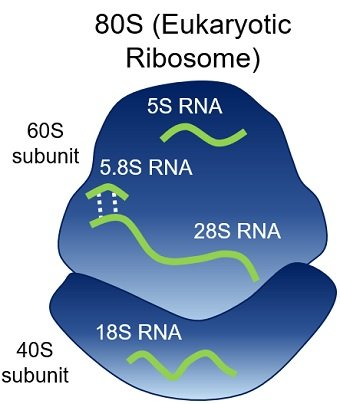
\includegraphics[width=0.2\textwidth]{80-S-ribosome.jpg}
    }
    \caption{Prokaryotic vs Eukaryotic Ribosomes}
\end{figure}

\section{Introduction}
DNA contains the genetic information that has instructions necessary for cells to function. The DNA that contains the codification of the amino acids chain necessary for a protein is copied to the messenger RNA (mRNA). The mRNA is formed in the nucleus and is then moved to the cytoplasm, where the ribosomes are located. The protein synthesis process is divided into four stages: initiation, elongation, termination, and recycling. In the initiation phase, the ribosome wraps around the mRNA and the tRNA. In the elongation phase, the ribosome reads the mRNA and decodes the sequence of nucleotides into a sequence of amino acids. In the termination phase, the ribosome finishes the protein synthesis process and releases the protein. In the recycling phase, the two subunits of the ribosome separate.

\section{Structure}
The ribosome has two subunits. The larger subunit has the role of putting together the amino acids to form the proteins, while the smaller subunit has the role of reading and decoding the mRNA. The ribosome contains ribosomal RNA (rRNA) and proteins, both of which are found in both the large and the small subunit. The role of the rRNA is to help with the binding of the mRNA and the tRNA, and to catalyze the peptide bond formation for the protein synthesis process. The role of the proteins is mostly a structural one, helping with the stability of the ribosome.

\begin{flushleft}
    \begin{figure}
        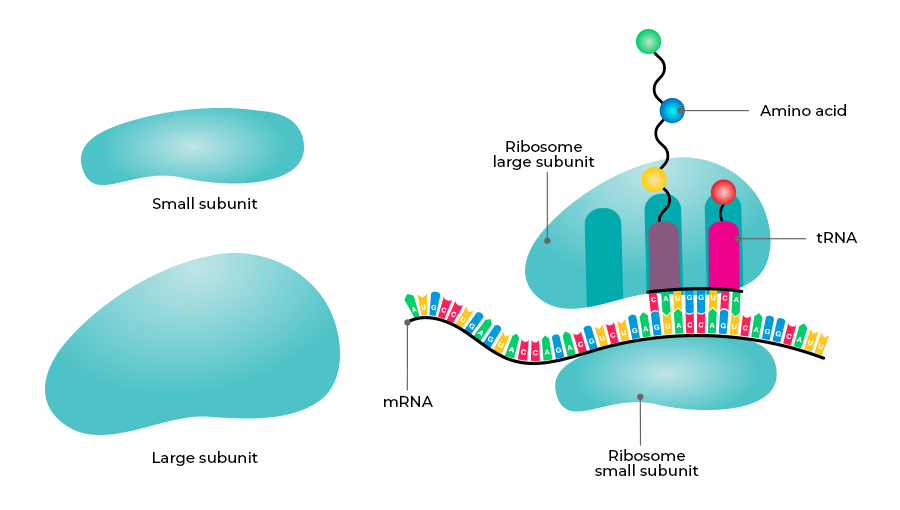
\includegraphics[width=0.7\textwidth]{Ribosome.png}
        \caption{Ribosome during the protein synthesis process}
    \end{figure}
\end{flushleft}

\section{Translation Process}
The translation process is the step in which the ribosome reads the mRNA and decodes it to find the correct sequence of amino acids to form a protein. The mRNA is made up of nucleotides. A nucelotide is a molucule that contains a nitrogen base, such as adenine (A), cytosine (C), guanine (G), or uracil (U). The ribosome reads the mRNA three nucleotides at a time, which is called a codon. Each codon corresponds to an amino acid in the tRNA. The start codon is always AUG, and the stop codon is either UAA, UAG, or UGA. These are the stop codons because there is no corresponding amino acid in the tRNA for them. The ribosome has three places for binding tRNA: the P site (peptidyl), the A site (aminoacyl), and the E site (exit). The A site is where the tRNA that carries the next amino acid that needs to be added to the protein enters. The P site is where the tRNA that contains the in-progress polypeptide chain is. The E site is where the tRNA that has finished its job goes to be released from the ribosome.

\section{Discovery}
Ribosomes were discovered by George Palade, a Romanian-American biologist, in the 1950s. He discovered them using an electron microscope, and were initially named Palade granules. They were later renamed ribosomes by Howard M. Dintzis in 1958. Palade won the Nobel Prize of Physiology or Medicine in 1974, alongside Albert Claude and Christian de Duve.

\section{Conclusion}
In conclusion, ribosomes are very important for all organisms, as they handle the protein synthesis process, which is essential for life.

\end{document}